\documentclass[conference,a4paper]{IEEEtran}
\IEEEoverridecommandlockouts
\usepackage[T1]{fontenc}
\usepackage{lmodern}
\usepackage{cite}
\usepackage{amsmath,amssymb}
\usepackage{graphicx}
\usepackage{booktabs,tabularx,array}
\usepackage{url}
\usepackage[hidelinks]{hyperref}
\usepackage{balance}
\usepackage{microtype}
\graphicspath{{../figures/}}
\setlength{\tabcolsep}{3.7pt}
\begin{document}
\title{Comparing Full Fine-Tuning and Low-Rank Adaptation of FLAN-T5 for Financial Sentiment Classification}
\author{\IEEEauthorblockN{Sampath Adimalla}
\IEEEauthorblockA{MSc Data Science and Computational Intelligence\\Coventry University, Coventry, United Kingdom\\Student ID: 17522555 \quad | \quad Module: 7043SCN}}
\maketitle
\begin{abstract}
This study investigates whether parameter-efficient adaptation can approach full fine-tuning (FFT) when a compact, instruction-tuned encoder--decoder model is specialised for financial news sentiment classification. Google FLAN-T5 Small was evaluated without task training and after supervised FFT or low-rank adaptation (LoRA). Financial PhraseBank's 75\%-agreement subset yielded 3,448 deduplicated sentences, partitioned into 2,412 training, 518 validation and 518 held-out test instances. Models were compared using macro F1, accuracy, class-level errors, paired bootstrap intervals, parameter counts, training resources and sensitivity to instruction wording. Test macro F1 increased from 0.3323 for the baseline to 0.9133 after FFT; the validation-selected LoRA rank-16 adapter reached 0.9085. LoRA trained 688,128 parameters rather than 76,961,152 and reduced recorded training time by 46.5\%. The paired 95\% bootstrap interval for the LoRA--FFT difference included zero. Nevertheless, rewording the inference instruction lowered macro F1 to 0.8087 for FFT and 0.6357 for LoRA. These findings indicate that efficient domain adaptation is feasible on modest hardware, but comparable standard-prompt accuracy does not imply comparable instruction robustness.
\end{abstract}
\begin{IEEEkeywords}
financial sentiment analysis, FLAN-T5, low-rank adaptation, parameter-efficient fine-tuning, domain adaptation, prompt sensitivity
\end{IEEEkeywords}

\section{Introduction}
Interpreting financial news involves contextual judgements that general-purpose sentiment methods can miss. A report of lower expenditure, for example, could signal improving efficiency or deteriorating investment. Financial PhraseBank was designed to capture economic sentiment from an investor perspective rather than relying on isolated positive and negative words \cite{malo2014}. Domain-adapted encoders such as FinBERT have consequently become important baselines for financial sentiment analysis \cite{araci2019}. The present investigation instead addresses the adaptation of a small \emph{generative} language model whose output is a sentiment label.

The text-to-text T5 formulation makes classification compatible with an encoder--decoder architecture \cite{raffel2020}; instruction fine-tuning subsequently improved the zero-shot usability of FLAN-family models \cite{chung2024}. Yet general instruction-following competence does not ensure reliable discrimination among negative, neutral and positive financial statements. Updating every model parameter may offer strong specialisation but has storage and compute implications. LoRA freezes the base weights and trains low-rank updates to selected projections \cite{hu2022}, an attractive option for limited GPU environments. Financial-domain systems such as FinGPT also demonstrate interest in accessible parameter-efficient adaptation \cite{yang2023}, although their data, objectives and model scales are not directly comparable with this experiment.

This study examines three questions: \emph{(1)} How far does supervised adaptation improve an untuned FLAN-T5 baseline? \emph{(2)} What predictive performance and resource trade-offs distinguish FFT from LoRA? \emph{(3)} Do conclusions about model quality remain stable when the test instruction is rephrased? The contribution is a controlled, prediction-level comparison, including an adapter-rank ablation, paired uncertainty estimates and a diagnostic prompt-sensitivity evaluation. The objective is robust empirical comparison, not a claim of state-of-the-art benchmark performance.

\section{Data and Language Model}
\subsection{Dataset provenance and preparation}
The study uses \emph{Financial PhraseBank}, specifically \texttt{Sentences\_75Agree}, in which at least 75\% of annotators agreed on the sentence's sentiment \cite{malo2014,phrasebank}. The original archive was read directly rather than relying on an older dataset-loading script. The downloaded source comprised 3,453 English news statements with negative, neutral or positive labels. Five duplicate sentences were removed before data splitting, leaving 3,448 records. A stratified partition using seed 42 produced the subsets in Table~\ref{tab:data}. The held-out test distribution is imbalanced: neutral accounts for 322/518 (62.2\%) observations. Class-averaged F1 was therefore designated the primary metric before test evaluation; accuracy alone can reward a majority-class predictor.

\begin{table}[!t]
\centering
\caption{Deduplicated dataset and stratified partitions}
\label{tab:data}
\begin{tabular}{lrrrr}
\toprule
Subset & Negative & Neutral & Positive & Total\\
\midrule
Training & 294 & 1,497 & 621 & 2,412\\
Validation & 63 & 322 & 133 & 518\\
Test & 63 & 322 & 133 & 518\\
\midrule
Overall & 420 & 2,141 & 887 & 3,448\\
\bottomrule
\end{tabular}
\end{table}

Rows were tracked using hashed sentence identifiers, and the exported manifests contain a source URL, archive digest and split assignments. No identifier occurs in multiple partitions. This eliminates exact duplicate overlap but does not preclude related company stories or topics appearing on both sides of the split. The selected high-agreement subset also excludes more ambiguous annotations; the results should not be taken as evidence of performance on all financial news.

\subsection{Model card and prediction task}
The model is \texttt{google/flan-t5-small} \cite{flant5hub}, a 76.96-million-parameter encoder--decoder Transformer. An instruction and financial sentence are supplied to its encoder, and the decoder generates one of three labels as text. Training targets are the literal strings \texttt{negative}, \texttt{neutral} and \texttt{positive}. Input and target lengths are capped at 128 and 8 tokens, respectively; inference permits up to six newly generated tokens. The same test items, standard prompt and greedy output-to-label conversion are applied to every model. Predictions outside the permitted label set would count as errors rather than be discarded; none occurred in the three main test runs. This is sentence-level classification, \emph{not} financial advice, price forecasting or portfolio optimisation.

\section{Fine-Tuning Methodology}
\subsection{Baseline, FFT and LoRA}
Four configurations were assessed. The \emph{baseline} uses the published checkpoint without gradient updates. \emph{FFT} updates every pretrained weight under a supervised, token-level cross-entropy objective. \emph{LoRA} keeps the pretrained matrices fixed while learning low-rank updates in the attention \texttt{q} and \texttt{v} projections. For a weight matrix $W$, adaptation has the form
\begin{equation}
W' = W + \frac{\alpha}{r} BA,
\label{eq:lora}
\end{equation}
where $A$ and $B$ are trainable low-rank factors, $r\in\{8,16\}$ and $\alpha=16$ \cite{hu2022}. Both adapters use dropout 0.05. Rank 8 trains 344,064 parameters, while rank 16 trains 688,128. These ranks constitute an explicit capacity ablation; no test label informed their selection.

All trained configurations use five epochs, training batch size 8, gradient accumulation factor 2, effective batch size 16, AdamW, 0.01 weight decay and warm-up ratio 0.10. Learning rates differ by method: $5\times10^{-5}$ for FFT and $3\times10^{-4}$ for LoRA. Checkpoints are retained according to the smallest recorded validation loss. Between the two adapter ranks, the selection criterion is \emph{validation macro F1}; rank 16 scored 0.8943, compared with 0.8899 for rank 8. Only the selected adapter was evaluated on the final test set. A common dataset split and evaluation prompt support comparison, although differing learning rates mean this is a comparison of practical training recipes rather than an isolated effect of parameter freezing.

\subsection{Evaluation and uncertainty}
For class $c$, $F1_c=2P_cR_c/(P_c+R_c)$, and the primary score is
\begin{equation}
\operatorname{MacroF1}=\frac{1}{3}\sum_{c\in\{-,0,+\}}F1_c.
\end{equation}
Secondary measures are accuracy, class-wise precision and recall, confusion matrices, training wall time, trainable parameters and peak PyTorch-allocated GPU memory. The main test estimates use 1,000 non-parametric bootstrap resamples over the 518 paired predictions, with percentile 95\% intervals \cite{efron1993}. For pairwise contrasts, the \emph{same sampled row indices} are applied to both models in each resample, preserving the paired design. These intervals quantify variation from resampling test examples, not across independently trained model initialisations.

A further exploratory test replaced the standard classification instruction with a semantically similar alternative while preserving all 518 held-out sentences and label definitions. No model was retrained or selected using this alternative prompt. This is an instruction-fragility test, not a temporal or cross-dataset generalisation benchmark.

\section{Experimental Setup}
The experiments were executed on Google Colab with one NVIDIA Tesla T4 (14.56\,GiB reported memory), Python 3.13.16, PyTorch 2.11.0+cu130, Transformers 4.57.1, PEFT 0.18.0 and scikit-learn 1.7.2. Seed 42 was used for data splitting and training. The run configuration requested BF16; because T4 lacks native BF16 tensor-core arithmetic, this setting must not be interpreted as evidence of native BF16 acceleration. Each trained run recorded 755 optimiser steps. GPU values reported below represent the framework's peak \emph{allocated} memory, not total device occupancy, reserved memory or hardware requirements across all environments.

The baseline and trained models were evaluated on identical row identifiers. The source manifest, package versions, checkpoint-selection records, prediction CSVs and training histories were retained. They allow independent recalculation of test metrics, although the lightweight evaluation export does not contain full model weights; reproducibility of training requires the accompanying notebook and saved checkpoints. All quantitative claims in the following section are taken from the executed experiment files, rather than from expected or simulated results.

\section{Results}
\subsection{Held-out classification performance}
Table~\ref{tab:results} and Fig.~\ref{fig:f1} show substantial gains from both adaptations. Baseline accuracy was 0.3378 and macro F1 was 0.3323; importantly, the baseline predicted no neutral test sentences correctly despite neutral being the dominant class. Its accuracy was also below a trivial always-neutral classifier (0.6216 on these data). The poor untuned result thus demonstrates a mismatch between the tested zero-shot instruction and the domain-specific label task, not an intrinsic limit of all pretrained language models.

\begin{table}[!t]
\centering
\caption{Locked-test metrics, $n=518$ (standard prompt)}
\label{tab:results}
\begin{tabular}{lrrrr}
\toprule
Model & Accuracy & Macro F1 & 95\% CI & Errors\\
\midrule
Untuned & 0.3378 & 0.3323 & [0.299,0.364] & 343\\
FFT & \textbf{0.9189} & \textbf{0.9133} & [0.882,0.940] & 42\\
LoRA ($r=16$) & 0.9170 & 0.9085 & [0.877,0.935] & 43\\
\bottomrule
\end{tabular}
\end{table}

\begin{figure}[!t]
\centering
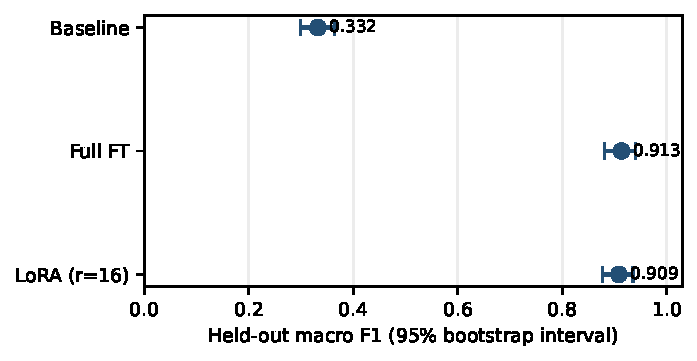
\includegraphics[width=\columnwidth]{f1_ci.pdf}
\caption{Observed macro F1 and 95\% percentile bootstrap intervals on the locked test set.}
\label{fig:f1}
\end{figure}

FFT attained 0.9133 macro F1, while LoRA reached 0.9085, a raw difference of 0.0048. The paired bootstrap estimate of LoRA minus FFT was $-0.0050$, with interval $[-0.0214,0.0094]$. Since this interval includes zero, the data do not establish a reliable advantage for either adaptation under this particular resampling analysis. Prediction disagreement was limited to nine of 518 cases; FFT made 42 errors and LoRA made 43. Neutral was classified most accurately, while positive statements were harder: positive-class F1 was 0.8561 (FFT) and 0.8476 (LoRA).

\subsection{Efficiency and learning dynamics}
\begin{table}[!t]
\centering
\caption{Recorded training resource comparison}
\label{tab:eff}
\begin{tabular}{lrrr}
\toprule
Quantity & FFT & LoRA $r=8$ & LoRA $r=16$\\
\midrule
Trainable parameters & 76.96M & 0.344M & 0.688M\\
Train time (s) & 360.30 & 192.82 & 192.87\\
Peak allocated GPU (GiB) & 1.747 & 0.750 & 0.757\\
Best val. loss & 0.0925 & 0.1035 & 0.1021\\
\bottomrule
\end{tabular}
\end{table}

Relative to FFT, selected LoRA updated 99.11\% fewer parameters, required 46.5\% less recorded training wall time and reduced recorded peak allocated GPU memory by 56.7\% (Table~\ref{tab:eff}). These measures arise from one T4 session; they are not formal energy-consumption or deployment-cost measurements. The loss trajectories in Fig.~\ref{fig:loss} show decreasing training loss across the three trained models. LoRA's modest rank-16 validation advantage should not be overstated, given one seed and the small difference between ranks.

\begin{figure}[!t]
\centering
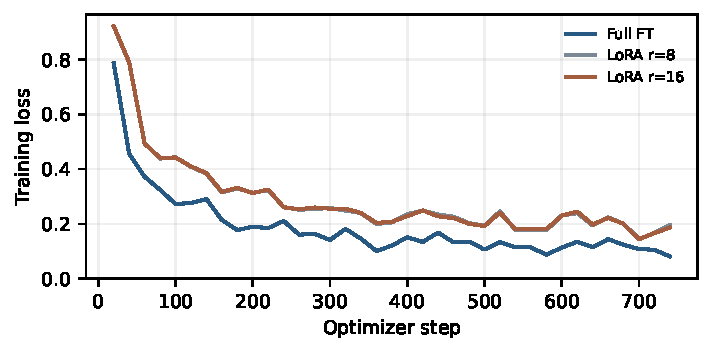
\includegraphics[width=\columnwidth]{loss_curves.pdf}
\caption{Recorded training loss against optimiser steps; all three runs completed 755 steps.}
\label{fig:loss}
\end{figure}

\subsection{Prompt robustness as a failure mode}
The alternative instruction materially changed the evaluation. FFT macro F1 dropped from 0.9133 to 0.8087 (10.46 percentage points), whereas LoRA fell from 0.9085 to 0.6357 (27.28 points); the untuned model declined to 0.2319. Figure~\ref{fig:prompt} illustrates the difference. None of these changes reflects a different test corpus or invalid-label rate; they arise from changed instruction phrasing. This result qualifies the favourable standard-prompt efficiency trade-off: the selected adapter was more instruction-sensitive in this particular test. Because only one additional phrasing was tried, the experiment identifies a warning sign rather than an estimated average over possible prompts.

\begin{figure}[!t]
\centering
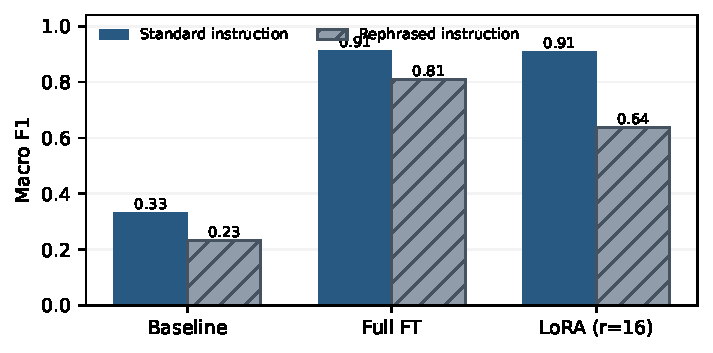
\includegraphics[width=\columnwidth]{prompt_f1.pdf}
\caption{Macro F1 on the same 518 test sentences under two instruction formulations.}
\label{fig:prompt}
\end{figure}

\section{Discussion, Applicability and Limitations}
The findings answer the first two research questions in a qualified way. Task-specific supervision transformed FLAN-T5 Small from a poor zero-shot classifier into a high-scoring held-out classifier. LoRA then approached FFT accuracy while updating substantially fewer weights and shortening training. This agrees with the motivation for parameter-efficient adaptation \cite{hu2022}, but it does not imply universal equivalence: the recipe, corpus size and validation-selected rank constrain the comparison. The third question produces the most consequential qualification. Small changes to the instruction exposed markedly greater fragility in LoRA than in FFT, despite their similar standard-prompt F1 scores.

Four limitations influence interpretation. First, training was run with one seed; the bootstrap intervals cannot replace repeated training to assess optimisation variability. Second, sentence-level random splits permit shared entities, lexical patterns and news themes, making independently sourced or time-separated evaluation necessary. Third, the agreement-filtered corpus is short, historical and biased towards unambiguous sentences, whereas operational pipelines encounter ambiguous, lengthy and rapidly changing information. Fourth, the prompt study compared only two manually chosen instructions; controlled prompt families and testing under label-preserving paraphrases would provide a more credible robustness estimate. Calibration and abstention thresholds were also outside scope because the model was evaluated as a generative discrete-label predictor, not as a reliable probability estimator.

\subsection{Social, ethical, legal and professional considerations}
In practice, an efficient classifier could assist with indexing financial news, triaging documents or analyst review, but not autonomously authorise trading or regulated advice. A positive label is a textual interpretation, not a prediction of future returns. Operational use would require human oversight, data-shift monitoring, quality review on contemporary news, confidence and abstention testing, and procedures for contested labels. The publicly distributed dataset carries CC BY-NC-SA 3.0 conditions, which should govern attribution and any reuse or redistribution of its text \cite{phrasebank}; derived result exports alone should not be confused with unrestricted rights over the source corpus. Model cards and versioned evaluation records should disclose the observed prompt dependence and intended-use boundary.

\section{Conclusion}
On 518 held-out Financial PhraseBank examples, full fine-tuning raised FLAN-T5 Small's macro F1 from 0.3323 to 0.9133. Validation-selected LoRA reached 0.9085 with far fewer trainable parameters and shorter training time. The paired bootstrap interval did not establish a dependable performance difference between the adapted models. Rephrased instructions, however, produced substantial degradation, especially for LoRA. The defensible conclusion is that LoRA offers an effective \emph{standard-prompt} efficiency option, while further multi-seed, temporal and prompt-robust evaluation is required before stronger real-world claims.

\balance
\begingroup\small
\begin{thebibliography}{12}
\bibitem{malo2014} P. Malo, A. Sinha, P. Korhonen, J. Wallenius, and P. Takala, ``Good debt or bad debt: Detecting semantic orientations in economic texts,'' \emph{J. Assoc. Inf. Sci. Technol.}, vol. 65, no. 4, pp. 782--796, 2014, doi: 10.1002/asi.23062.
\bibitem{araci2019} D. Araci, ``FinBERT: Financial sentiment analysis with pre-trained language models,'' arXiv:1908.10063, 2019. [Online]. Available: \url{https://arxiv.org/abs/1908.10063}
\bibitem{raffel2020} C. Raffel \emph{et al.}, ``Exploring the limits of transfer learning with a unified text-to-text transformer,'' \emph{J. Mach. Learn. Res.}, vol. 21, no. 140, pp. 1--67, 2020.
\bibitem{chung2024} H. W. Chung \emph{et al.}, ``Scaling instruction-finetuned language models,'' \emph{J. Mach. Learn. Res.}, vol. 25, no. 70, pp. 1--53, 2024.
\bibitem{hu2022} E. J. Hu \emph{et al.}, ``LoRA: Low-rank adaptation of large language models,'' in \emph{Proc. Int. Conf. Learn. Represent. (ICLR)}, 2022. [Online]. Available: \url{https://arxiv.org/abs/2106.09685}
\bibitem{yang2023} H. Yang, X.-Y. Liu, and C. D. Wang, ``FinGPT: Open-source financial large language models,'' arXiv:2306.06031, 2023. [Online]. Available: \url{https://arxiv.org/abs/2306.06031}
\bibitem{phrasebank} P. Malo \emph{et al.}, ``Financial PhraseBank,'' dataset release hosted by Hugging Face. [Online]. Available: \url{https://huggingface.co/datasets/takala/financial_phrasebank} (accessed Oct. 2026).
\bibitem{flant5hub} Google, ``FLAN-T5 Small,'' model card, Hugging Face Model Hub. [Online]. Available: \url{https://huggingface.co/google/flan-t5-small} (accessed Oct. 2026).
\bibitem{efron1993} B. Efron and R. J. Tibshirani, \emph{An Introduction to the Bootstrap}. London, U.K.: Chapman \& Hall, 1993.
\end{thebibliography}
\endgroup

\vspace{0.3em}
\noindent\textit{Word count (abstract and main text, excluding headings, captions, tables and references): 1,914.}
\end{document}
